%%%%%%%%%%%%%%%%%%%%%%%%%%%%%%%%%%%%%%%%%%%%%%%%%%%%%%%%%%%%%%%%%%%%%%%%
\chapter{MBT in agilen Entwicklungsumgebungen}
\label{sec:problemdescription}
%%%%%%%%%%%%%%%%%%%%%%%%%%%%%%%%%%%%%%%%%%%%%%%%%%%%%%%%%%%%%%%%%%%%%%%%

\section{Fallstudie: Kundenberaterapplikation bei Raiffeisen Schweiz}

\subsection{Hintergrund zu den Applikation RETo und RESi}
Die Applikation \textit{RESi}, in anderer Struktur und bis in das Jahr 2013 \textit{RETo} (Raiffeisen Expert Tool), ist ein Backend-Service der Dienste für die verschiedensten Front-End Applikationen des Unternehmens bereitstellt. Unter altem Namen, bot die Applikation früher eine eigene Benutzeroberfläche und weniger, dafür spezifischere Funktionalität. RETo war im Intranet der Fillialen im Einsatz und wurde ausschließlich für Kundenberatungen eingesetzt. Die Applikation hatte folgende Kernkompetenzen:

\begin{itemize}
\item Ermittlung von Anlegerprofilen
\item Durchführung von Anlage-Checks
\item Beratungen zum Thema Wohnen und Wohneigentum
\item Beratungen zum Thema Vorsorge
\item Beratungen zum Thema Pension
\end{itemize}

Im Jahr 2014 wurde ein Großteil der Applikationslandschaft umstrukturiert. In einer Bemühung einzelne Applikationen zu vereinheitlichen und Mehrfachaufwendungen zu minimieren, wurde RETo modularisiert. Das Projekt RESi wurde gestartet. RESi stellt eine Back-End-Service Schicht dar. Da RETo bereits einen sehr breiten Funktionsumfang bot, besteht RESi zu großen Teilen aus den RETo Kernkomponenten. Auch das Entwicklungsteam ist das selbe geblieben. Mehrere, ehemals eigenständige Applikationen, greifen jetzt auf RESi zu und bieten nur noch ein Front-End und eine dünne Serverschicht. RETo existiert weiterhin aber greift auch auf die Services von RESi zu.

\subsection{Entwicklungsumfeld}
Das Umfeld er Applikaiton RESi wird in einem klassischen Auftragnehmer/Auftraggeber Szenario entwickelt. Eine Fachabteilung stellt den Kunden dar. Sie definieren die Anforderungen an die Applikation. Dem gegenüber ist das Entwicklungsteam. Dieses besteht aus einem Applikationsmanager und 6-8 Entwicklern. 

\begin{itemize}
\item 2 Major Release pro Jahr
\item Mehrere Service-Release pro Jahr
\item 3-wöchige Scrum-Sprints
\item 4 Ebenen (Integrationstest, Systemtest, Akzeptanztest, Produktion)
\item Scrum Master wechselt
\item Product Owner (PO) wird von Fachbereich gestellt
\item tägliche Scrum-Meetings
\end{itemize} 

Die Applikation RESi ist, bedingt durch ihre Reife, bereits sehr stabil. Effektiv ist sie schon seit mehreren Jahren (in anderer Struktur und unter anderem Namen) im produktiven Einsatz. Der typische Entwicklungszyklus wird also vom Fachbereich angestoßen. Ein Request For Change (RFC) wird vom Fachbereich angenommen oder verfasst. Die zuständigen Produktmanager definieren genügend fachliche Details, bevor ein RFC in eine Story verwandelt wird. Diese Story fließt nun typischerweise in den Scrum-Backlog (\todo{Ref zu Scrum Kapitel}). Wenn auf einer der Entwicklungsebenen Fehler mit hoher Priorität gefunden werden, wird ein Defect-Bericht verfasst, der direkt in den laufenden Entwicklungszyklus (Sprint) einfließt.\\
Auf Seiten der Entwickler finden kurze tägliche Meetings statt. Dauer und Struktur dieser täglichen Meetings entsprechen den klassischen Daily-Scrum Standups. Neben den Entwicklern ist der Scrum-Master und der Product Owner aus dem Fachbereich anwesend. Er steht für kurzfristig auftretende Fragen bereit. Weiters finden im Entwicklungsteam wöchentliche Research-Meetings statt. In diesen werden die neu eingetroffenen Stories analysiert und modularisiert. Ziel ist es, eine Story in Tasks herunterzubrechen, die in einem Arbeitstag schaffbar sind. Ein Task soll also von einem einzelnen Entwickler implementiert werden. Im selben Zug, wird werden die Aufwände der Story und damit der Tasks geschätzt. Im RESi Team kommen zwei verschiedene Methoden zur Aufwandsschätzung zum Einsatz. Einerseits wird eine Methode verwendet wo alle Stories offen und ungeordnet aufgelegt werden. Nun wird das Team der Reihe nach gebeten, eine Story einzuordnen. Damit werden weder Storypoints noch Stunden geschätzt. Stories werden anhand ihrer augenscheinlichen Aufwänden geordnet. Wenn kein Teammitglied mehr eine Änderung machen will, endet die Aufwandsschätzung. Der Scrum-Master legt schlussendlich, in Absprache mit dem Team, fest welcher Bereich von Stories einen zukünftigen Sprint fließen. Nimmt man Stories aus dem vorderen Bereich der Reihung, mindert dies den Gesamtaufwand viel höher als wenn Stories aus dem hinteren Teil zurück in den Backlog verschoben werden. 

\subsection{Entwicklungsebenen}
Zwischen der Implementierung eines Tasks und dessen Eintritt in eine produktive Umgebung, läuft dieser durch definierte Ebenen. Während der Bearbeitung eines Tasks, benutzen die Entwickler eine lokale Installation der Applikation (diese entspricht der Ebene \textit{Integrationstest}). Wenn ein Entwickler einen Task abschließt und alle Unit-Tests erwartungsgemäß durchlaufen werden, wird der Task zum \textit{Code Review} freigegeben. Ein anderer Entwickler liest den Code und gibt Feedback zu Richtigkeit, Effizienz, Lesbarkeit und Stil des Code-Stücks. Das Code-Stück wird, nach eventueller Korrektur, auf der Ebene \textit{Integrationstest} deployed (ein IBM WebSphere Applikationsserver \footnote{IBM WebSphere \url{http://www.ibm.com/websphere}} im Falle von RESi). Diese Ebene hat die Hauptaufgabe, auftretende Nebeneffekte aufzudecken, die das neu programmierte Code-Stück verursacht. Ab diesem Zeitpunkt beginnt der Fachbereich bereits mit manuellen Tests auf dem Integrationsserver. In manchen Fällen macht es keinen Sinn gegen einen einzelnen Task zu testen (möglicherweise lässt er sich GUI-seitig auch gar nicht testen). Dann wird abgewartet bis sich verwandte Tasks oder die ganze zugehörige Story für den Integrationsserver freigegeben werden. Da Entwickler und Fachbereich täglich auf dieser Ebene arbeiten, werden auftretende Nebeneffekte durch Wartungsänderungen eher entdeckt.\\
Nach Abschluss eines Sprints wird der Stand der Ebene \textit{Integrationstest} auf \textit{Systemtest} deployed. Hier testet der Fachbereich genau definierte Abläufe. Außerdem unternimmt eine gesonderte Test-Abteilung Last- und Performance Tests auf dieser Ebene. Bis zu diesem Zeitpunkt läuft die Entwicklung relativ streng nach agilen Prinzipien. Um das Zusammenspiel der Applikationslandschaft zu vereinheitlichen, wird unternehmensweit aber immer noch auf viel längere Release-Zyklen gesetzt. Sprint-Ergebnisse werden also nicht zeitnah in die Produktionsebene versetzt. Die Ebene \textit{Akzeptanztest} wird also zwischen Systemtest und \textit{Produktionsebene} gezogen. Auf ihr werden die Stände getestet, die für Major-Releases geplant sind. Typischerweise wird gegen Ende eines Major-Release Zyklus verstärkt auf der Ebene \textit{Akzeptanztest} deployed und getestet. Trotzdem kann es zu Überlappungen kommen die mit dem agilen Iterationszyklus interferieren. Sprint-Ergebnisse die kurz vor einem Major-Release eigentlich für produktionsreife getestet werden sollten, werden möglicherweise erst für die nächste Veröffentlichung beachtet. Erstens werden also Testressourcen periodisch für \textit{Akzeptanztest} benötigt, obwohl bereits neuere Versionen der Applikation testbar wären. Zweitens leidet das Endprodukt wenn Features, die eigentlich zur Veröffentlichung freigegeben werden könnten, mehrmonatige Verspätungen haben.

\subsection{Qualitätssicherung im Projekt}
In Entwicklung und Qualitätssicherung des Produkts sind diverse Parteien involviert. Anfänglich, also zum Zeitpunkt der Requirementanalyse und der Spezifikationsentwicklung, sind auch Teams eingeklinkt die während der Maintenance-Phase nicht mehr beteiligt sind. Dazu zählen auch externe Mitarbeiter.\\
Während der Maintenance-Phase des Systems gibt es einen Test-Verantwortlichen. Diese Rolle befindet sich auf Seiten der nicht-technischen Produktmanager. Der Test-Verantwortliche delegiert und orchestriert die Erstellung und Durchführung von manuellen Testfällen. Alle Teams benutzen zum Requirements- und Testmanagement HP QualityCenter \footnote{HP QualityCenter Internetauftritt \url{http://www8.hp.com/us/en/software-solutions/quality-center-quality-management/}}. Dies hat den Vorteil, dass übergreifend alle Beteiligten über den Status des Produkts genau informiert sind. Manuelle Testfälle und Testfallsuiten sind meist textuell beschrieben und manchmal als COS-Tabellen (Conditions of Satisfaction) definiert. Diese COS-Tabellen haben eine hohe Ähnlichkeit zu Skripts die beim Einsatz von automatisierten GUI-Tests zum Einsatz kommen (siehe Abbildung \ref{fig:cos_raiffeisen}).

\begin{figure}[h] 
  \centering
     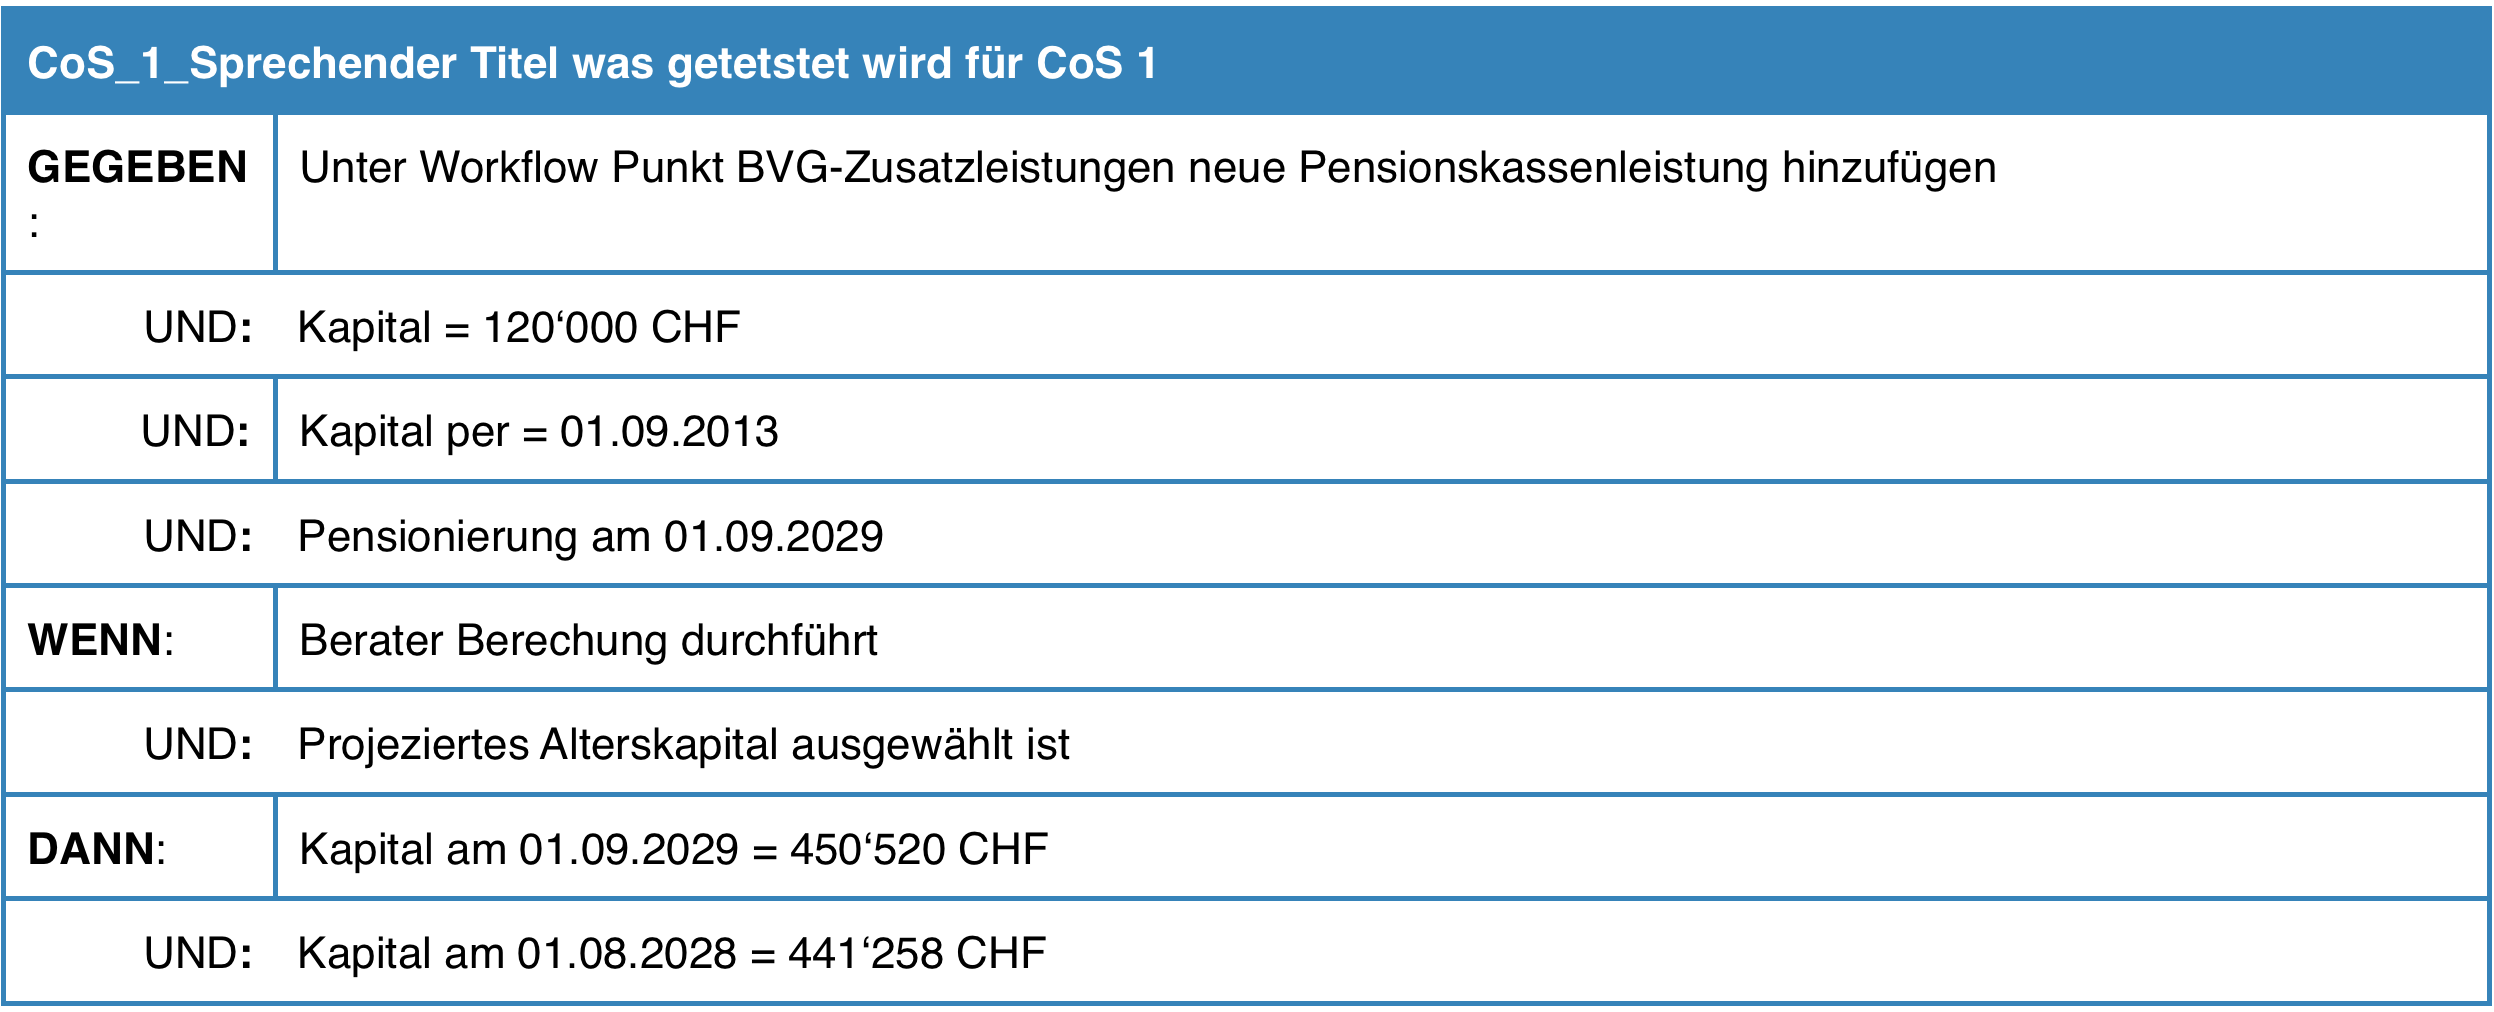
\includegraphics[width=0.9\textwidth]{figures/cos_raiffeisen.png}
  \caption{Muster-COS Tabelle wie sie von den Testfalldesignern verwendet werden.  Angegeben werden Pre- sowie Postconditions und die auszuführenden Aktionen. Der Detailgrad kann erheblich variieren.}
  \label{fig:cos_raiffeisen}
\end{figure}


Auf Seiten der Entwickler, also im Scrum-Team, gibt es keinen dedizierten Tester. Im Entwicklungszyklus fixiert sind nur Unit-Tests. Außerdem werden vom Test-Verantwortlichen auch den Entwicklern manuelle Testfälle zugewiesen die im Rahmen vom Integrationstesting durchgeführt werden.

\subsubsection{Erkannte Schwachstellen in der Qualitätssicherung}
-Viele Beteiligte
-Keine klare Zuständigkeiten
-Hohe Diversität bei eingesetzten Tools
-Testfalldesign nicht transparent
\subsubsection{Versuch der Qualitätssicherung durch skriptgesteuerte GUI-Tests}

\subsubsection{Aufwendige Wartung von Testdaten}
Tracing von Testdaten und Testfällen (welcher Bereich der Testdaten wird von einem bestimmten Testfall benutzt?). `If data is tightly coupled with behaviour, this can lead to serious maintenance burden' \cite{baker_model-driven_2005} 
\subsubsection{Abhilfe durch Modellbasiertes Testen der Schnittstellen?}

%%%%%%%%%%%%%%%%%%%%%%%%%%%%%%%%%%%%%%%%%%%%%%%%%%%%%%%%%%%%%%%%%%%%%%%%

\section{MBT auf Unit-Testebene}
\subsection{ModelJUnit}
ModelJUnit wird von Dr. Mark Utting et al. an der Universität Waikato in Neuseeland entwickelt. Es wird unter der Open Source GNU GPL Lizenz entwickelt und befindet sich zur Zeit in der Version 2.5 \footnote{Homepage des Tools ModelJUnit \url{http://www.cs.waikato.ac.nz/~marku/mbt/modeljunit/}}. Es erlaubt die Modellierung des SUT als endlicher Automat (von hier an FST für \textit{finite state machine}) in Java, Generierung von Testfällen laut spezifiziertem Traversierungsalgorithmus sowie Reporting. Seit Version 2.0 bietet das Tool eine grafische Benutzeroberfläche die die Traversierungskonfiguration ermöglicht und veranschaulicht.\\
\todo{Hier weitermachen aus Utting Buch}
\subsubsection{Traversierung}
\paragraph{Random Walk}
\paragraph{Greedy Walk}
\paragraph{Lookahead Walk}
\paragraph{Quick Walk}


\section{MBT auf Integrationstestebene}
\subsection{Testing von Serviceorientierten Architekturen mittels UML Testing Profile}

\subsubsection{UML Testing Profile BASICS}

\subsubsection{SOA und Web-Services}
Von Serviceorientierten Architekturen (von hier an \textit{SOA}) verspricht man sich schnelle und einfache Integration innerhalb als auch über Unternehmensgrenzen hinweg. Die Möglichkeit eine Applikation mittels Komposition, maßgeschneidert zu den gegebenen Requirements, zusammenzustellen, ist traditionellen Software-Engineering Methoden oft voraus. Gleichzeitig stellen verschachtelte und unabhängige Strukturen den Tester vor neue Herausforderungen. \\
SOA wird missbräuchlich oft mit Web-Services gleichgestellt. Tatsächlich sind Web-Services nur die häufigste architektonische Grundlage auf der SOA-Applikationen laufen. Die folgende Sektion geht ebenfalls von einer Serviceorientierten Architektur basierend auf Web-Services aus.

\subsubsection{Mapping von Web-Service Elementen auf UML-Diagramme}
Am Beispiel eines Web-Services der per WSDL\footnote{WSDL Web-Service Spezifikationssprache 2.0 \url{http://www.w3.org/TR/wsdl20/}} definiert ist, soll gezeigt werden wie eine Modellierung von Web-Services mittels dem UML-Testing Profile umgesetzt werden kann. \footnote{Sehr ähnlich würde eine Modellierung für RESTful Web-Services basierend auf WADL ausschauen. Hierbei stellt sich aber eine Grundsatzfrage: Eines der Prinzipien von REST ist die Fähigkeit, dass sich ein Web-Service selbst beschreiben kann. Inwiefern trotzdem WADL Dateien gebraucht werden, hängt von der jeweiligen Implementierung ab.} Baker et al. schlagen folgende Vorgehensweise für das Mapping vor\cite{_model-driven_2007}:

\begin{itemize}
\item WSDL Port Types werden zu UML Stereotyp-Klassen gemappt
\item Die Operationen in dieser Klasse stellen die Operationen dar, die der jeweilige Port Type offenbart.
\item Jede Operation hat eine übereinstimmende Request Message. Falls die Operation auch einen Rückgabewert definiert, wird auch dieser abgebildet.
\item Komplexe Typen als auch Enumerationen werden zu stereotypisierten Klassen.
\end{itemize}

\subsubsection{Teststrategie für Web Services}
Im Gegensatz zu herkömmlichen Desktop-Applikationen aus einer Hand, können SOA Web-Services tief verschachtelte Komponenten von verschiedensten Parteien enthalten. Dies erschwert das Testing auf zwei Arten. Erstens können gravierende Qualitätsunterschiede zwischen Web-Services bestehen. Zweitens unterliegen diese benutzten Web-Services eigenen Wartungs- und Änderungsintervallen. Diese Erkenntnisse haben zur Folge, dass an die Teststrategie für Web-Services folgende zusätzliche Anforderungen gestellt werden:

\begin{itemize}
\item Tests müssen schnell und oft durchführbar sein (nämlich dann wenn eine Komponente geändert wird): \textit{On-Demand Testing}.
\item Gleichzeitig müssen die Tests kompakt und schnell wartbar sein (ähnlich Unit-Tests).
\item Web-Services sollen einzeln getestet werden können. Dies ermöglicht nicht nur eine gewisse Modularität, die zu einer hohen Test-Geschwindigkeit beiträgt sondern erleichtert auch die Fehlersuche einem negativen Testdurchlauf.
\end{itemize}

Web-Services müssen \textit{mehrdimensional} getestet werden\cite{_model-driven_2007}. Das bedeutet, ein modellbasierter Testfall soll alle Port Types, die der Service zur Verfügung stellt, kombiniert mit allen Operationen die jeder Port Type anbietet, prüfen. Als Testdaten müssen die Equivalenzklassen aller Datentypen die der Web-Service anbietet identifiziert werden.

\subsubsection{Beispielhafte TestSuite eines SOA Web-Services}
\todo{UML-Diagramme (und evt. WSDL)aus Buch einbinden} In diesem Beispiel wird ein Service einer Bücherei oder einer Buchhandlung herangezogen. Einfachheitshalber bietet dieser Service nur einen Port Type (LibraryService) an. Auf diesem werden drei Operationen angeboten (search, reserve, fetch). Ein Client kann ein Element aus dieser Bücherei also suchen und basierend auf seinem Status-Parameter handeln. Das Element kann sofort verfügbar, später verfügbar und nicht lokal verfügbar sein.\\

Um die angesprochene mehrdimensionale Abdeckung zu gewährleisten bietet das UML Testing Profile das Konzept der Data Pools.\todo{Ref zu Kapitel UTP}. Der DataPool stellt das kartesische Produkt dar, dass aus Operationen und Datenelementen gebildet wird. Nun kann ein Testtreiber auf diesem DataPool operieren und auf Testfalldiagramme (UML-Sequenzdiagramme) referenzieren.\\
Anhand von diesem einfachen Beispiel wird sichtbar, dass das UML Testing Profile sinnvolle Erweiterungen definiert, die die Modellierung von modernen SOA-Applikationen vereinfachen. Data Pools visualisieren die Abdeckung von Äquivalenzklassen und modularisierte Sequenzdiagramme erlauben die Modellierung von umfangreichen Testfällen. 


\subsubsection{Ausfühhrung von UTP Tests mittels JUnit}
Agile Praktiken haben die Wahrnehmung der die Wichtigkeit des Unit-Tests erhöht\cite{_model-driven_2007}. Ansätze wie \textit{Test-First} sind in diesem Umfeld besonders populär und der klassische Unit-Test spielt dabei eine zentrale Rolle. Dieses Kapitel geht davon aus, dass der Leser mit den Grundlagen von JUnit 4\footnote{Webseite des JUnit Projekts \url{http://junit.org/}} vertraut ist.\\

Zum Zeitpunkt dieser Arbeit, gibt es keine Tool mit welchem die automatische Generierung von JUnit-Testfällen aus UTP-Modellen erlaubt. Das bedeutet, um MBT basierend auf UTP-Modellen in einem realen Umfeld zu betreiben, muss das Mapping manuell gemacht werden. Baker et al. schlagen dabei folgende Vorgehensweise vor\cite{_model-driven_2007}:

\begin{table}[h]

\centering
\begin{tabular}
{ | l |p{9cm}|} \hline
\textbf{UTP} & \textbf{JUnit} \\ \hline
SUT                       & Kein direktes Mapping nötig. Jede Klasse im \textit{Classpath} kann angesprochen und getestet werden   \\ \hline
Kontext                   & Kein direktes Mapping. JUnit kann auf den realen Kontext des SUT zugreifen. Aufwände außerhalb der JUnit-Programmierung sind nötig um alternative Konfigurationen zu testen \\ \hline
Ablauf         			  & JUnit bietet die Klasse \textit{org.junit.runner.Runner} um feingradige Einstellungen am Testablauf zu machen. \\ \hline
Sheduler                  & Alle vom Java-Umfeld bereitgestellten Möglichkeiten des Shedulings sind einsetzbar (auch \textit{org.junit.runner.Runner} bietet Sheduling-Optionen) \\ \hline
Test configuration        & Implizit gegeben in JUnit, durch die direkte Einbindung der Klassen die getestet werden. \\ \hline
Test objective            & Dieses Konzept bietet JUnit nicht. Methoden können höchstens mit entsprechenden Kommentaren versehen werden.\\ \hline
Test case                 & Eine Methode die mit der Annotation \textit{@Test} versehen ist. \\ \hline
Test invocation           & Aufrufe der Methoden die mit \textit{@Test} annotiert sind. Üblicherweise durch einen Test-Runner. \\ \hline
Arbiter                   & Die Klassen \textit{org.junit.runner.Runner} und \textit{org.junit.runner.notification.RunListener} entscheiden über die Bewertung des Ausgangs eines Testfalls. Diese Klassen können bei Bedarf auch erweitert werden. \\ \hline
Verdict                   & Vordefinierte Testfallergebnisse sind \textit{pass},\textit{fail} und \textit{error}. Auch diese Klasse kann um mehr Funktionalität erweitert werden. \\ \hline
Defaults                  & JUnit bietet keinen vergleichbaren Mechanismus.  \\ \hline
Validation action         & Validation Actions mappen auf die vielfältigen Methoden der Klasse \textit{org.junit.Assert} \\ \hline
Stimulus and observation  & Keine entsprechende Funktionalität in JUnit. \\ \hline
Logging concepts          & Im Java-Umfeld gibt es verschiedenste Logging-Frameworks die mit JUnit verwendet werden können. \\ \hline
Testdatenmanagement: Data pools & \textbf{Es sind keine entsprechenden Konzepte in JUnit eingebaut.} \\ \hline
Testdatenmanagement: Wildcards  & Es sind keine entsprechenden Konzepte in JUnit eingebaut.\\ \hline
Timer                     & Es sind keine entsprechenden Konzepte in JUnit eingebaut. \\ \hline
Timezone                  & Es sind keine entsprechenden Konzepte in JUnit eingebaut. \\ \hline
Deployment       & JUnit fügt sich im Deployment Prozess sehr gut ein. \\ \hline
\end{tabular}
\caption{Mapping von UTP zu JUnit}
\end{table}

\todo{UTP zu JUnit Code Beispiel einfügen eventuell}
UTP wurde entwickelt um mit JUnit zusammenzuspielen\cite{_model-driven_2007}. Tatsächlich lassen sich viele Konzepte gut von UTP-Modellen nach JUnit übertragen. Gleichzeitig hat die Ausführung von UTP-Testfällen in JUnit gravierende Schwächen.

\paragraph{Manuelles Mapping} Es hat sich in den Jahren, seit das UML Test Profile veröffentlicht wurde, keine Community um die Nutzung und Entwicklung von Tools gebildet. Die Eigenentwicklung eines JUnit-Testfallgenerators kann im Umfeld von großen Softwareprojekten sinnvoll sein. Gleichzeitig bleibt der Aufwand um den sogenannten \textit{glue code} zu schreiben (also die Implementierungsdetails innerhalb der Testmethoden).\\
Jedenfalls können durch einen manuellen Eingriff neue Fehler entstehen. Ein Modell mittels Testfällen umzusetzen ist kein trivialer Vorgang und erfordert genaue Kenntnisse des Frameworks sowie des SUT. Ob sich die Modellierung und die Aufwände für die Umsetzung in JUnit-Testfällen lohnt, lässt sich schwer feststellen. Faktisch bietet die Modellierung als UTP-Diagramm zwar strukturierte Testfälle (verglichen mit der Ad-Hoc Entwicklung von JUnit-Testfällen) aber keine weiteren Qualitätsmetriken. Entwicklungsumgebungen und statische Code-Analyse Tools können die Abdeckung von JUnit-Testfällen eruieren, diese ist in agilen Softwareprojekten aber ohnehin schon sehr hoch. Ein modellbasierter Ansatz kann hier wenig belegbare Qualitätsvorteile schaffen.

\paragraph{Keine Unterstützung der Testdatenmangementkonzepte}
Vor allem das \textit{Data Pool} Konzept von UTP ist eine Notwendigkeit für datenintensive Applikationen. Datengetriebene Testfälle müssen durch ein flexibles und zuverlässiges Konzept gestützt werden. Auch hier müsste eine Eigenentwicklung gemacht werden. Diese ist aber nicht nur aufwendig sondern stellt sich auch die Frage der Zukunftssicherheit. Kann das Modul zum Testdatenmanagement mit anderen Technologien verwendet werden oder ist es zu stark auf UTP zugeschneidert?

\subsection{Schnittstellentests mit Graphwalker}
Graphwalker\footnote{Graphwalker 3 Website inklusive Dokumentation \url{www.graphwalker.org}} ist ein Open Source MBT-Tool zur Online- und Offline Generierung von Testsequenzen aus Endlichen Automaten (siehe Abschnitt \ref{sec:fsm}) sowie Erweiterten Endlichen Automaten (EFSM).Graphwalker ist in Java und JavaScript implementiert und bietet eine Java-API an. Das Graphwalker-Projekt wurde von zwei Entwicklern der Firma Spotify, Nils Olsson und Kristian Karl, gegründet. Bei Spotify, dem marktführenden Musik-Streaming-Service, ist das Tool auch stark im Einsatz. Graphwalker ist zur Zeit (Frühjahr/Sommer 2015) aktiv unter Entwicklung und liegt bereits in der Version 3.0 vor.\\
Graphwalker weicht ab vom herkömmlichen Testfall-Workflow. Das SUT wird in einem Modell (Graph) modelliert und das Testing (also die Traversierung des Graphs) wird vom gewählten Algorithmus und dessen Konfiguration bestimmt. Daraus resultieren lange, unvorhersehbare Testdurchläufe. Die offizielle Dokumentation beschreibt es so:

\begin{quote}
`We do not want to walk the same path every time we execute a test. We want variation, spiced with randomness. This will create a better `test coverage' of the system under test.'\cite{_graphwalker_2015}
\end{quote}

Beim Einsatz in den agilen Entwicklungsteams von Spotify hat sich gezeigt, dass diese Testdesign-Philosophie sehr gut in die kurzen Entwicklungsiterationen passt. Weiters eignen sich die simplen FSM-Diagramme sehr gut um Feedback von Stakeholdern einzuholen, weil sie auch ohne technischen Hintergrund verständlich sind.

\subsubsection{Modellierungs-Syntax}
Graphwalkers Modellierungssprache basiert nicht auf UML, weil die Autoren glauben, dass Tester vom großen Funktionsumfang von UML nicht brauchen und abgeschreckt werden. Stattdessen setzt Graphwalker auf GraphML\footnote{Website des GraphML Projekts \url{graphml.graphdrawing.org}}. GraphML setzt nicht auf eine proprietäre Syntax sondern basiert auf herkömmlichen XML-Dateien und wird unter der \textit{Creative Commons Attribution 3.0}-Lizenz entwickelt.\\
Zur Erstellung von Modellen in GraphML, mit denen Graphwalker umgehen kann, eignet sich jedes Tool, das GraphML-Dateien exportieren kann. Das von den Entwicklern empfohlene Tool ist \textit{yEd}\footnote{Website der Firma yWorks und des yEd Graph Editors \url{http://www.yworks.com/en/products/yfiles/yed/}}, welches völlig kostenlos verwendet werden kann. yEd bietet eine simple Benutzeroberfläche und für die Erstellung von Modellen für Graphwalker ist nahezu kein Einarbeitungsaufwand vorhanden.\\
Modelle in Graphwalker sind gerichtete Graphen. Knoten repräsentieren einen Zustand in dem sich das SUT befindet. Kanten beschreiben die Aktion die zu einem bestimmten Zustand führen. Graphwalker ignoriert grafische Attribute der Modelle wie Farbe und Liniendicke der Elemente. Üblicherweise finden in den Knoten die Überprüfungen (\textit{Assertions}) und in den Kanten die Befehle (Klicks, Schnittstellenaufrufe...) statt. Kanten müssen in Graphwalker genau eine Richtung haben. Es folgt eine kurze Beschreibung der Möglichkeiten, die die Syntax von Graphwalker bietet um die Traversierung der Graphen, und damit der Testfälle, zu beinflussen.

\paragraph{Start vertex} Wenn ein Startknoten definiert wird, darf es nur genau einen geben. Es ist aber nicht obligatorisch einen Startknoten zu definieren.

\paragraph{Guards} Auf Kanten könnten sogenannte \textit{Guards} definiert werden. Dabei handelt es sich um einen Konditionalmechanismus. Wenn das Konditional zu wahr evaluiert, wird die Kante traversierbar. Ein \textit|{Guard} wird mittels eckigen Klammern beschrieben.
\begin{verbatim}
[loggedIn == true]
\end{verbatim}

\paragraph{Actions} Auch \textit{Actions} sind nur auf Kanten definierbar. Hierbei handelt es sich um Code in JavaScript-Syntax der zur Zeit der Traversierung ausgeführt wird. Die in \textit{Actions} durchgeführten Zuweisungen werden in \textit{Guards} abgefragt.

\paragraph{Keywords} Diese Schlüsselwörter beschreiben keine Eigenschaften des SUT, sondern dienen nur der Usability und Modularität der Modelle.


\begin{itemize}
\item Start: Beschreibt den Startknoten
\item BLOCKED: Dieser Knoten oder diese Kante wird bei der Traversierung aus dem Graphen entfernt.
\item SHARED: Dient zur Modularisierung. Wenn Graphwalker bei der Traversierung auf einen mit SHARED annotierten Knoten trifft, passiert ein Sprung in ein anderes Modell mit dem selben SHARED-Bezeichner.
\item INIT: Dient zur Initialisierung von Datenfeldern die im Modell genutzt werden. Nur Knoten können mit dem INIT-Schlüsselwort versehen werden.
\end{itemize} 

\paragraph{Modularisierung der Modelle}
Das SUT kann in Graphwalker mittels mehreren Modellen abgebildet werden. Dies hat mehrere Vorteile. Einerseits vereinfacht die Modularisierung eines großen Modells die Les- und Wartbarkeit. Andererseits wird dadurch die Wiederverwendbarkeit von Teilen der Funktionalität ermöglicht. Ein klassisches Beispiel ist ein Login-Workflow. Dieser kann oft zu mehreren Zeitpunkten bzw. an mehreren Stellen im SUT erfolgen. Statt das Modell aufzublähen oder mit zahlreichen Beziehungen schlechter lesbar zu machen, kann auf eine andere GraphML-Modelldatei verwiesen werden.\\
Graphwalker ermöglicht dies mit Sprüngen in andere Modelle. Wenn es bei der Traversierung auf einen Knoten mit dem Schlüsselwort \textit{SHARED} und einem Bezeichner stößt, kann ein Sprung in ein anderes Modell erfolgen, das einen Knoten mit dem selben Bezeichner hat (siehe Abbildung \ref{fig:gw_multiple_models}). Wenn nun mehrere Kanten zur weiteren Traversierung in Fragen kommen, entscheidet der Zufall ob in das andere Modell gesprungen wird.\\
Weiters ist zu erwähnen, dass die Modelle nicht einfach nur verflacht (\textit{flattening}) werden. Das bedeutet, dass die Modelle unabhängige Gültigkeitsbereiche haben. Die Traversierung erfolgt also in einem eigenen Kontext.

\begin{figure}[h] 
  \centering
     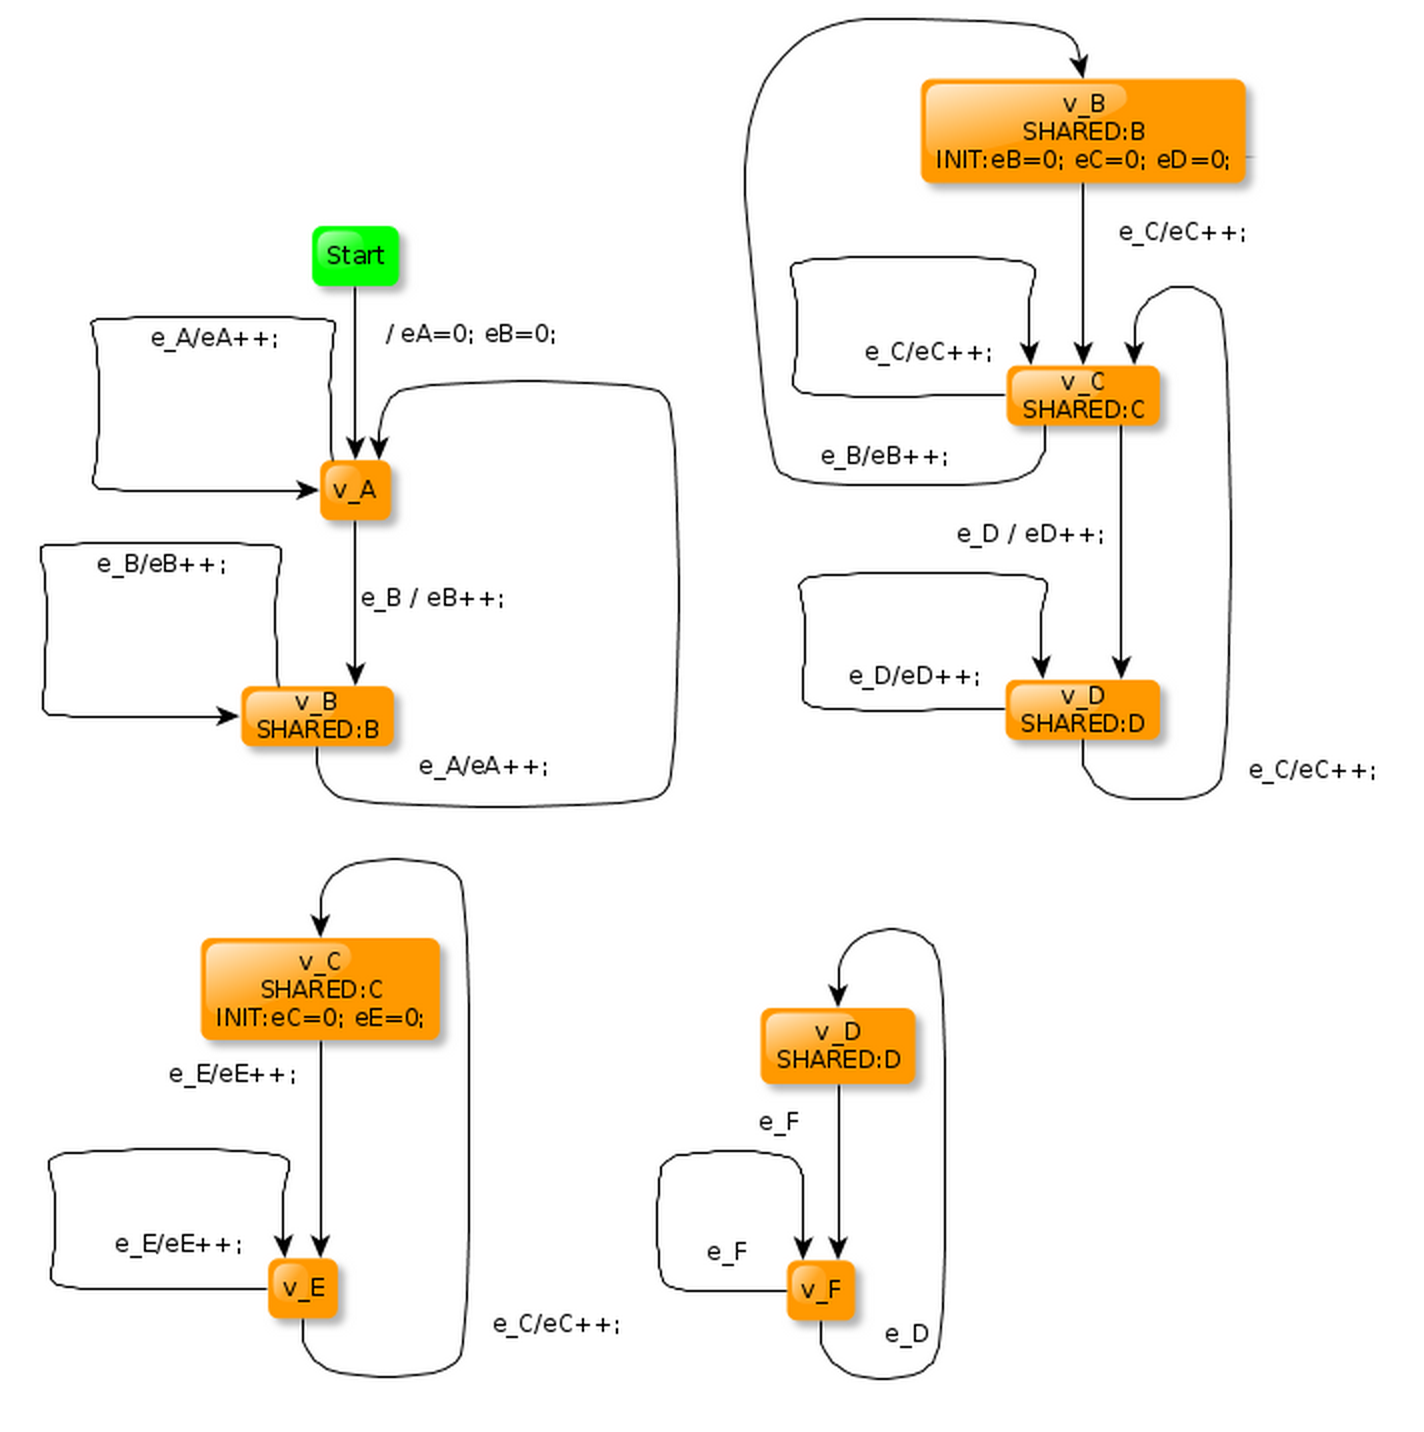
\includegraphics[width=0.9\textwidth]{figures/gw_multiple_models.png}
  \caption{Vier einzelne Modelle die bei einer Traversierung (ausgehend vom Startknoten in Grün) erreicht werden können. Bei den Knoten die mit \textit{SHARED} gekennzeichnet sind kann ein Sprung (und auch ein Sprung zurück) erfolgen. Die Variablen mit den selben Bezeichnern in den Modellen B und C befinden sich in unabhängigen Gültigkeitsbereichen.\cite{_graphwalker_2015}}
  \label{fig:gw_multiple_models}
\end{figure}

\paragraph{Traversierung der Modelle}  
Wie im ursprünglichsten Sinn des modellbasierten Tests, kennt Graphwalker das Konzept der Testfälle nicht. Das SUT wird als gesamtes oder nur zu Teilen modelliert und das Testing wird durch die Auswahl eines Traversierungsalgorithmus angestoßen. Da die meisten Traversierungsalgorithmen von einer randomisierten Variante abhängen, wird das SUT bei jedem Testdurchlauf leicht unterschiedlich traversiert und damit getestet.\\
Durch die Modellierung des Modells und der Auswahl sowie Einstellung eines Traversierungsalgorithmus kann also bestimmt werden wie das SUT getestet werden soll. Dabei bietet Graphwalker bereits verschiedenste Algorithmen an, die sich für unterschiedliche Testzwecke eignen. Die meisten dieser Algorithmen basieren auf bekannten Graph-Algorithmen und bieten, durch die quelloffene Entwicklung, volle Transparenz gegenüber dem Tester.

\subparagraph{Schnelle Traversierung - Smoke Tests}
Vor allem während der Testfallentwicklung und um sogenannte \textit{Smoke Tests} zu machen eignet sich der A*-Algorithmus von Graphwalker. Er basiert auf dem bekannten A*-Suchalgorithmus von Hart et al. \cite{hart_formal_1968}. Dabei wird also ein zu findender Knoten angegeben, meist ein Knoten der das Ende eines Workflows darstellt. Graphwalker durchschreitet das Testsystem dann in einem möglichst kurzen Pfad, wobei die zugrundeliegende Suchheuristik bei jedem Schritt angepasst wird.

\begin{verbatim}
@Test
public void runSmokeTest() {
    
    setPathGenerator(new AStarPath(new ReachedVertex("v_Browse")))
    
}
\end{verbatim}


\subparagraph{Traversierung basierend auf Pfadabdeckung - Funktionaler Test}
Umfangreiche funktionale Tests einer komplexen Applikation, wie sie beispielsweise über Nacht gemacht werden, können mit Graphwalker unter anderem durch eine Zufallstraversierung mittels Angabe der gewünschten Pfadabdeckung realisiert werden. Falls eine einhundertprozentige Abdeckung eingestellt wird (wie im folgenden Beispiel), wird das Modell vom Startknoten (falls angegeben) aus traversiert bis jede begehbare Kante traversiert wurde. Gegegebenenfalls werden weitere Durchläufe gestartet, falls es Teilgraphen gibt die vom designierten Startknoten nicht erreichbar sind. 

\begin{verbatim}
@Test
public void runFunctionalTest() {
    
    setPathGenerator(new RandomPath(new EdgeCoverage(100)))
    
}
\end{verbatim}


\subparagraph{Traversierung mit Zeitangabe}\todo{weitermachen...}


\subsection{Einbindung SoapUI/HP UFT}


\section{MBT auf Systemtestebene und Test non-stop}
\subsection{Manuelle Systemtests anhand von Modellen}
\subsection{Automatisierte MBT GUI-Tests (GUITAR)}
\subsection{Automatische Modellgenerierung auf Produktionsebene (LearnLib)}